% Template for IGARSS-2020 paper; to be used with:
%          spconf.sty  - LaTeX style file, and
%          IEEEbib.bst - IEEE bibliography style file.
% --------------------------------------------------------------------------
\documentclass{article}
\usepackage{spconf,amsmath,epsfig}
\usepackage{bbm,bm}
\usepackage{natbib}
\usepackage{graphicx}
\usepackage{subcaption}
\usepackage{amsmath}

% Example definitions.
% --------------------
\def\x{{\mathbf x}}
\def\L{{\cal L}}

% Title.
% ------
\title{Measuring and Enhancing the Visual Content of Polarimetric Synthetic Aperture Radar Decompositions}

\twoauthors
  {Ulil\'e Indeque \sthanks{Email: ui@laccan.ufal.br}}
  {Laborat\'orio de Computa\c c\~ao Cient\'ifica \\e An\'alise Num\'erica\\
  	Universidade Federal de Alagoas, Brazil
  }
{Alejandro C.\ Frery\sthanks{Email: alejandro.frery@vuw.ac.nz}}
   	{School of Mathematics and Statistics\\
   		Victoria University of Wellington, New Zealand
   	}
  
   	
\begin{document}
%\ninept
%
\maketitle
%
\begin{abstract}
Polarimetric Synthetic Aperture Radar images provide important information about the scene under observation.
There are several ways in which such information can be extracted, among them the visualization of polarimetric decompositions.
A polarimetric decomposition extracts features which, in principle, are related to basic components of the scene.
Its visualization depicts such components as variations in hue and intensity, but its interpretation may be hampered by low contrast.
Several image enhancement techniques may be applied to improve such a representation, but they may hamper the information contents.
We propose an approach for such enhancement based on the visual content that does not alter the interpretability of color images based on polarimetric decompositions and, at the same time, enhances the user's ability to extract visual information.
The technique also provides a quantitative measure of such visual content.
\end{abstract}
%
\begin{keywords}
Image enhancement;
Information content;
Polarimetric decompositions;
SAR Polarimetry;
Stochastic distances.
\end{keywords}
%
\section{Introduction}
\label{sec:intro}

Polarimetric Synthetic Aperture Radar (PolSAR) images have a prominent role in remote sensing \citep{PolarisationApplicationsRemoteSensing,LeePottier2009PolarimetricRadarImaging}.
Such images are formed by the return from the scene in several combinations of transmitting and receiving polarization of the electromagnetic waves.

The observation in each pixel of a fully polarimetric image is a $2\times2$ complex-valued matrix:
\begin{equation}
\bm S' = \begin{pmatrix}
   	S_{\text{HH}} & S_{\text{HV}}\\
   	S_{\text{VH}} & S_{\text{VV}}
\end{pmatrix}, \label{Eq:ScatteringMatrix}
\end{equation}
in which $S_{ij}$ is a complex value, and $i$ and $j$ are any of the two possible orientations: $\text{H}$ (horizontal) or $\text{V}$ (vertical).
Under the reciprocity principle, $S_{\text{HV}}=S_{\text{VH}}$, so the information in the scattering matrix~\eqref{Eq:ScatteringMatrix} can be encoded in the scattering vector
\begin{equation}
\bm S = \begin{pmatrix}
   	S_{\text{HH}}\\
   	S_{\text{HV}}\\
   	S_{\text{VV}}
\end{pmatrix}
\end{equation}
without loss of information.

More often than not, users employ multilooked images, in which $L$ ideally independent observations are averaged:
\begin{equation}
\bm Z = \frac{1}{L} \sum_{\ell=1}^L \bm S(\ell) \bm S^\dag(\ell),
\end{equation}
where ``$\dag$'' denotes the transpose of the complex conjugate.
With this, the multilook observation in each pixel has the form
\begin{equation}
\bm Z = \begin{pmatrix}
I_{\text{HH}} & \text{Cov}(S_{\text{HH}},S_\text{HV}) & \text{Cov}(S_{\text{HH}},S_\text{VV}) \\
\text{Cov}^*(S_{\text{HH}},S_\text{HV}) & I_{\text{HV}} & \text{Cov}(S_{\text{HV}},S_\text{VV})\\
\text{Cov}^*(S_{\text{HH}},S_\text{VV}) & \text{Cov}^*(S_{\text{HV}},S_\text{VV}) & I_{\text{VV}}
\end{pmatrix},
\label{Eq:Multilook}
\end{equation}
in which ``$*$'' denotes the complex conjugate, the diagonal elements are intensities, and the off-diagonal entries are the complex covariances between channels.
Except from a scale, \eqref{Eq:Multilook} is know as the coherence matrix.
There are other forms of storing the polarimetric return, among them the Pauli and the Kennaugh decompositions.
These representations are related, and it is relatively simple to transform one into another.

It is not possible to visualize directly observations of the form~\eqref{Eq:Multilook}, as they belong to $\mathbbm R_+^3\times \mathbbm C^3$, i.e., they are nine-dimensional objects.
Such observations encode valuable information from the target, and it is desirable to extract and visualize it.
Such extraction can be accomplished using Decomposition Theorems.

%\subsection{Decompositions Theorems}

PolSAR decomposition consists in retrieving the components which gave rise to each observation.
The purpose of such operation is to identify the average scattering mechanism within each pixel.
%In the following, we will summarize the main theorems for incoherent observations.

\citet{ModelingandInterpretationofScatteringMechanismsinPolarimetricSyntheticApertureRadarAdvancesandPerspectives2014} discuss the general additive decomposition framework
\begin{equation}
\bm Z = \sum_i^N \pi_i \bm Z^{(i)},
\end{equation}
in which $\bm Z^{(i)}$ is a prototypical scattering, 
$\pi_i$ the relative amount with which it contributes to the observation $\bm Z$, and $N$ is the number of components in the resolution cell.
Alternatively, \citet{APolSARScatteringPowerFactorizationFrameworkandNovelRollInvariantParametersBasedUnsupervisedClassificationSchemeUsingaGeodesicDistanceinpress} discuss a multiplicative rather than additive approach to this problem.

There are several well-known prototypical scatterers, whose form depends on the target.
Among them, we mention the volume, double bounce, odd bounce, and helix.
Their coefficients in an observation depends both on the target and on the sensing system conditions.

We are interested in decomposition theorems that naturally lead to visualization, i.e., that produce three components that can be mapped onto the red, green, and blue channels.
Examples of such decompositions are Barnes-Holmes, Pauli, Krogager, and Hyunen.

The dynamic range of the components values is typically very large, and the user has to choose how to map them into, usually, the $[0,255]$ interval in order to produce a pseudocolor image.
Typical mappings are the linear,
the trimmed linear,
and the equalization.
The linear mapping usually produces almost black images, while the trimmed linear requires stipulating a lower and upper bound.
Equalization has the advantage of producing values in $[0,1]$ which can be easily converted to $[0,255]$, but it may lead to color which are not related to the original ones.

A very popular visual enhancement technique is the spectral decorrelation.
It consists in computing the principal components of the original values (the decorrelation step), enhancing, and applying the inverse rotation.
This operation tends to produce crisp images with exaggerated contrast.

%\subsection{Information Content}

\citet{AssessingInformationContentinColorImages} proposed a technique for measuring the information content of color images with the Kullback-Leibler divergence between the observed and ideal histograms of the pixel values in the CIELAB color space.
This approach also allows improving an image's contrast by maximizing its realizable color information while retaining the chroma and hue.

In this paper, we propose a modified approach to measuring the visual information content in pseudocolor compositions obtained from decomposition theorems.
We also use our approach to enhance them without altering the information they encode.

\section{METHODOLOGY}
\label{sec:meth}
%The CIELab is an color space which presents an approximately uniform distribution and closer to human perception. To take advantage of it, image manipulation are performed with images encoded in CIELab color space. This paper aims to presents the technique to enhacing the image quality using matching histogram, manipulating the L component. The ideal image used as reference was generated randomly and has a uniform distribution. The observed images were generated by applying the Barnes-Holmes, Pauli, Krogager, and Hyunen decomposition algorithms.
%    By the way of the information content comparison, the Hellinger Distance which is an important metric in the fields of information theory is used to measure the distance between two probability distributions, which are: the L component histogram of the ideal and original image. 

%In this section, we will talk about the proposed technique to enhacing the images and the metric to assess the image quality.

The ideal image's values occupy regularly the CIELab color space.
Each pixel in an image in CIELab representation is of the form $I= (L, a, b)$, where 
$L\in[0,100]$ is the lightness (darkest to brightest), 
$a\in[-200,200]$ measures the color component from green to red, and 
$b\in[-200,200]$ describes the color component from blue to yellow.
This color representation, differently from the RGB and CMYK color spaces, approximates the human vision system.
\citet{AssessingInformationContentinColorImages} present and discuss the one-to-one conversions between color spaces.


%
%The originals image are denoted by $\bm {O=(r_O, g_O, b_O)}$ and encoded in the RGB color space. 
%These images are converted to CIELab color space having the components $\bm{O=(L_O, a_O, b_O)}$ and, in th final of operation, they are inversely converted to RGB color space, since they are inversible. The mapping from RGB to CIELab can be found in 

\subsection{Proposed approach}
\label{match}
The matching histogram technique consists in adjust the histogram of an image to be similar to another referenced image.

Consider two objects $I$ and $O$, respectively the ideal and original image.
The matching histogram function receives two object: the $H_{L_I}$ component as reference and the $H_{L_O}$ interest's object. 

The first step is equalization of $H_{L_O}$. 
This is done by applying the Empirical Cumulative Distribution Function - ECDF to the data.
This function is defined by 
\begin{equation}
    \bm F(t) = \frac1N\sum_{j=1}^N I(t_j \leq t) ,
    \label{eq:ecdf}
\end{equation}
the indicator $I$ is defined as
\begin{equation}
    \bm I(t_j \leq t) = \begin{cases}
        1,  & t_j \leq t \\
        0,  & t_j > t.
    \end{cases}
\end{equation}
Applying~\eqref{eq:ecdf} to $H_{L_O}$, we obtain the equalized image, denoted as $_eH_{L_O}$. 

The matching histogram can be obtained using the inverse empirical cumulative distribution function of $H_I$, applied to $_eH_{L_O}$
\begin{equation}
    \bm F^{-1}_{L_I}(_eH_{L_O}).
    \label{inv:cdf}
\end{equation}

From~\eqref{inv:cdf}, we have as result the histogram of $L_O$ component approximately equal to $H_{L_I}$. 
Using this component, we can reconstruct the original image $O$, replacing $H_{L_O}$ to $_aH_{L_O}$. 
Finaly, we have the enhanced original image formed by $O = (_aH_{L_O}, a_I, b_I)$ and converted back to RGB space color $O = (r_O, a_O, b_O)$.

The methodology is outlined in Fig.~\ref{Fig:Outline}.

\begin{figure*}
	\centering
	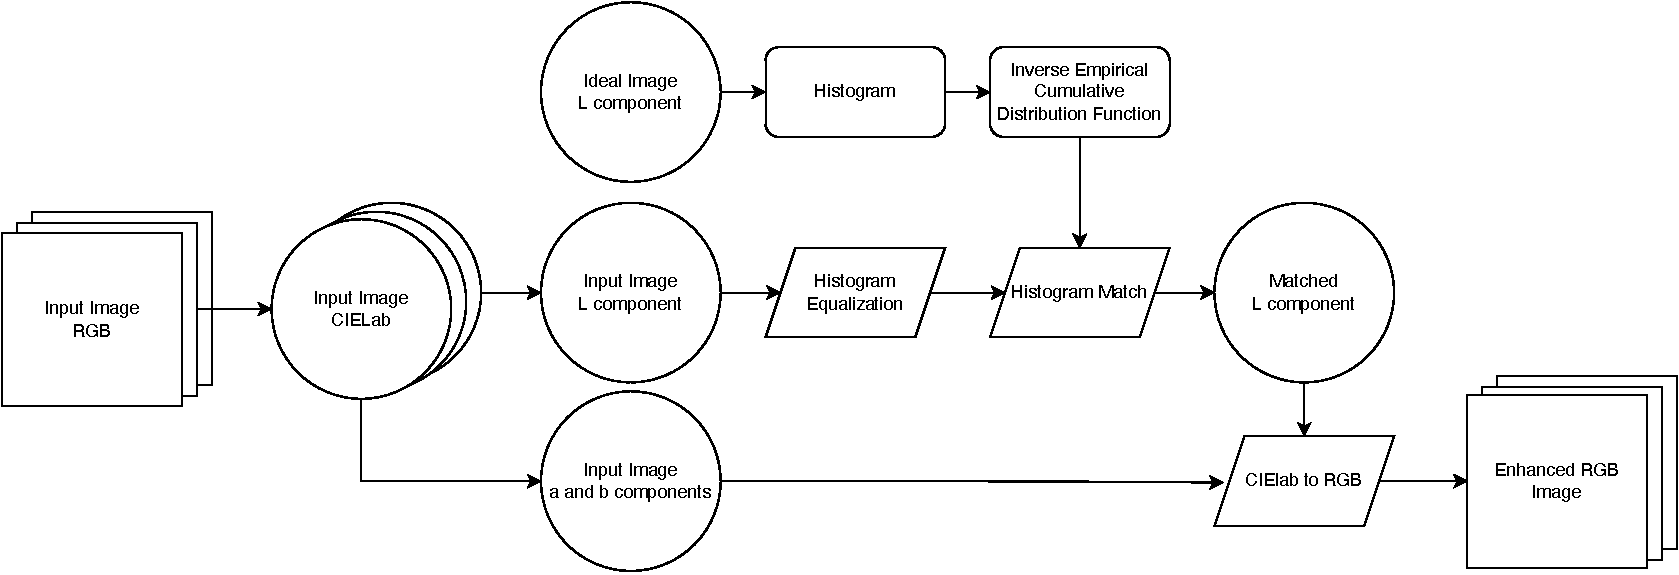
\includegraphics[width=.9\linewidth]{../../Diagrams/Outline}
	\caption{Outline of the enhancement procedure}\label{Fig:Outline}
\end{figure*}


\subsection{Evaluation Metrics}

An important point is to know how efficient the proposed technique is, i.e., a quantitative measure of the closeness of the results to the ideal image. 

This can be done by comparing the images histograms
There are several metrics that quantify the similarity between two probability distributions, among them the Kullback-Leibler divergence~\citep{AssessingInformationContentinColorImages}, and the
the Hellinger, 
Euclidean, and Canberra distances~\citep{BanchmarckSimiliraty}.
\citet{AssessingInformationContentinColorImages} used the Kullback-Leibler divergence in their proposal.

Consider the images $p(L, a, b)$ and $q(L, a, b)$.
The Kullback-Leibler divergences between the $p$ and $q$ channels
\begin{align}
D_{L}(p,q) & = \sum_{L} p(L) \log\frac{p(L)}{q(L)},\\
D_{a}(p,q) & = \sum_{a} p(a) \log\frac{p(a)}{q(a)},\\
D_{b}(p,q) & = \sum_{b} p(b) \log\frac{p(b)}{q(b)}.
\end{align}
The authors then propose adding these components divergences to obtain a measure of the difference between the images.
The Kullback-Leibler divergence is not necessary symmetric, and requires computing a ratio in which the denominator may be zero, and the logarithm of a quantity that may be zero.

The Hellinger distance is a widely used measure which does not have the problems metioned above.
It is defined as
\begin{equation}
	H(p, q) = \frac{1}{2}\sqrt{\sum_{j=1}^k \big(\sqrt{p_j} - \sqrt{q_j}\big)^2}.
\end{equation}
\citet{BanchmarckSimiliraty} computed the Hellinger distance along with other seven metrics, considering some factors such as complexity and the relationship with the amount of noise, and the Hellinger distance presented consistent and acceptable results.
We used the Hellinger distance to computed the dissimilarity between the images and the ideal signal.








\section{RESULTS}
\label{Sec:Results}

Fig.~\ref{Fig:Images} shows an original Pauli decomposition and a zoom (Figs.~\ref{Im:Original} and~\ref{Im:ZoomOriginal}),
the result of applying contrast enhancement by spectral decorrelation (Figs.~\ref{Im:Decorrelated} and~\ref{Im:ZoomDecorrelated}),
the version with equalized bands (Fig.~\ref{Im:Equalized} and~\ref{Im:ZoomEqualized}),
and the result of applying contrast improvement in the CIELab space (Figs.~\ref{Im:Enhanced} and~\ref{Im:ZoomImproved}).
The differences are noticeable.
While the three first have crisp and highly saturated colors, the last one is more realistic while preserving the hue.

\begin{figure*}[hbt]
\centering
\subcaptionbox{Original\label{Im:Original}}{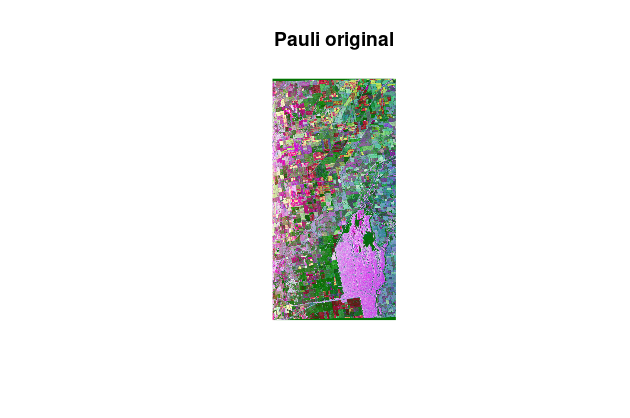
\includegraphics[width=.24\linewidth]{../image/pauli_original}}
\subcaptionbox{Decorrelated\label{Im:Decorrelated}}{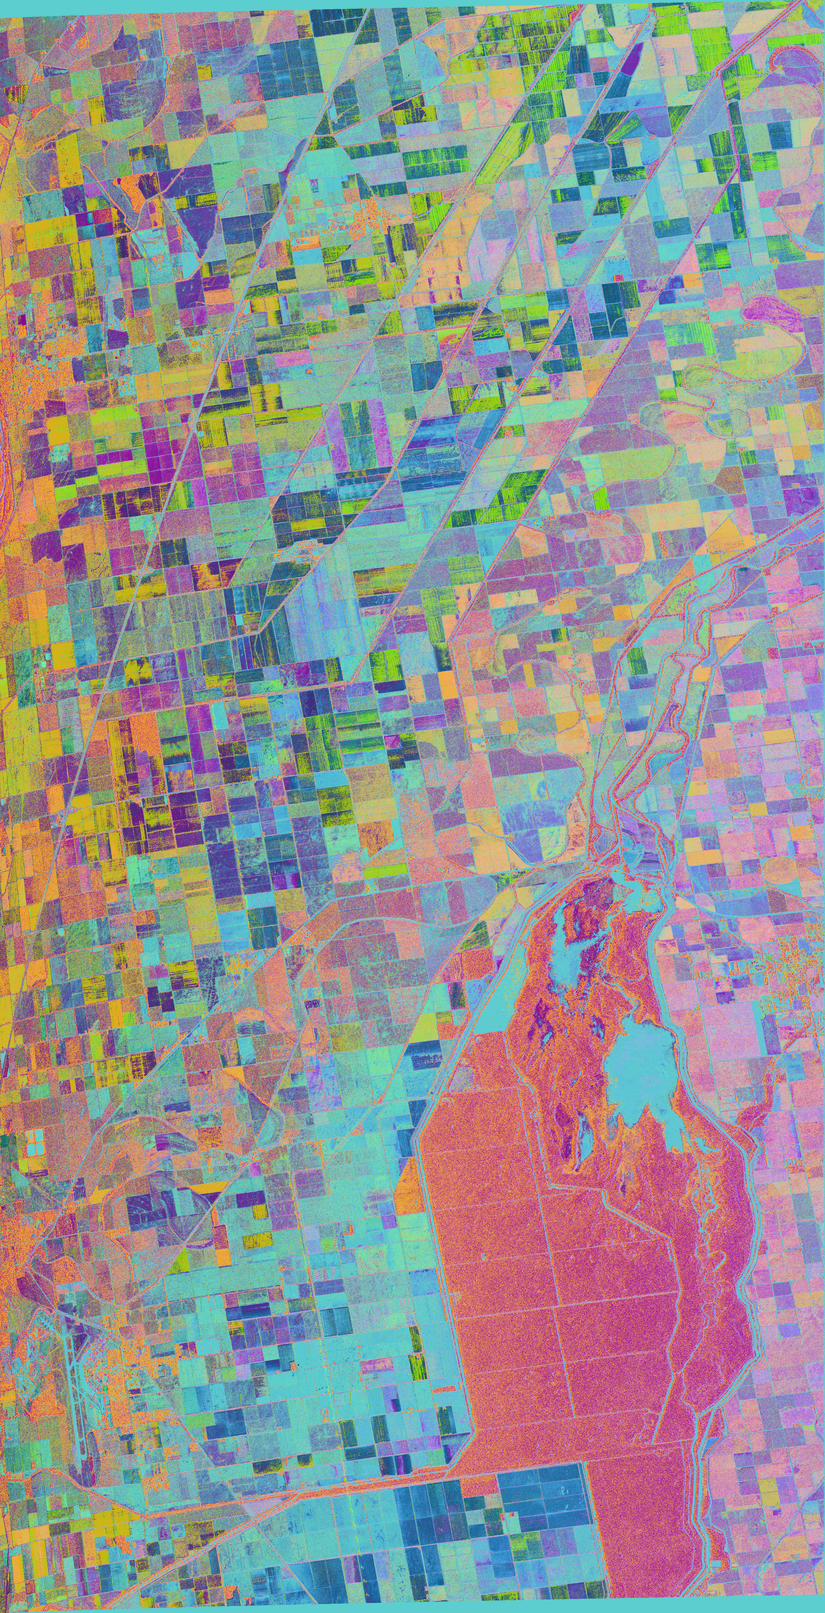
\includegraphics[width=.24\linewidth]{../image/pauli_decorr}}
\subcaptionbox{Equalized\label{Im:Equalized}}{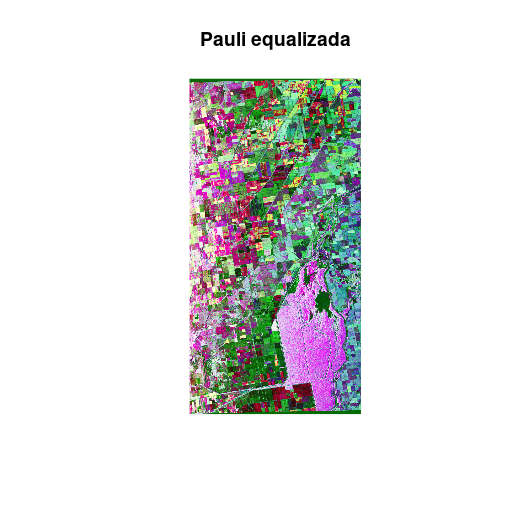
\includegraphics[width=.24\linewidth]{../image/pauli_equalizada}}
\subcaptionbox{Enhanced\label{Im:Enhanced}}{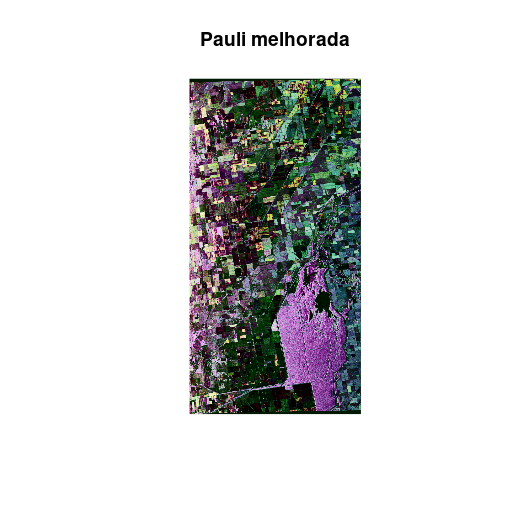
\includegraphics[width=.24\linewidth]{../image/pauli_melhorada}}
%
\subcaptionbox{Original zoom\label{Im:ZoomOriginal}}{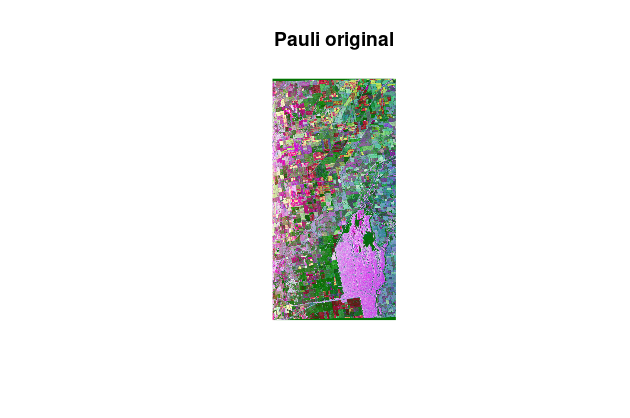
\includegraphics[width=.24\linewidth,viewport=575 600 825 850,clip]{../image/pauli_original}}
\subcaptionbox{Decorrelated zoom\label{Im:ZoomDecorrelated}}{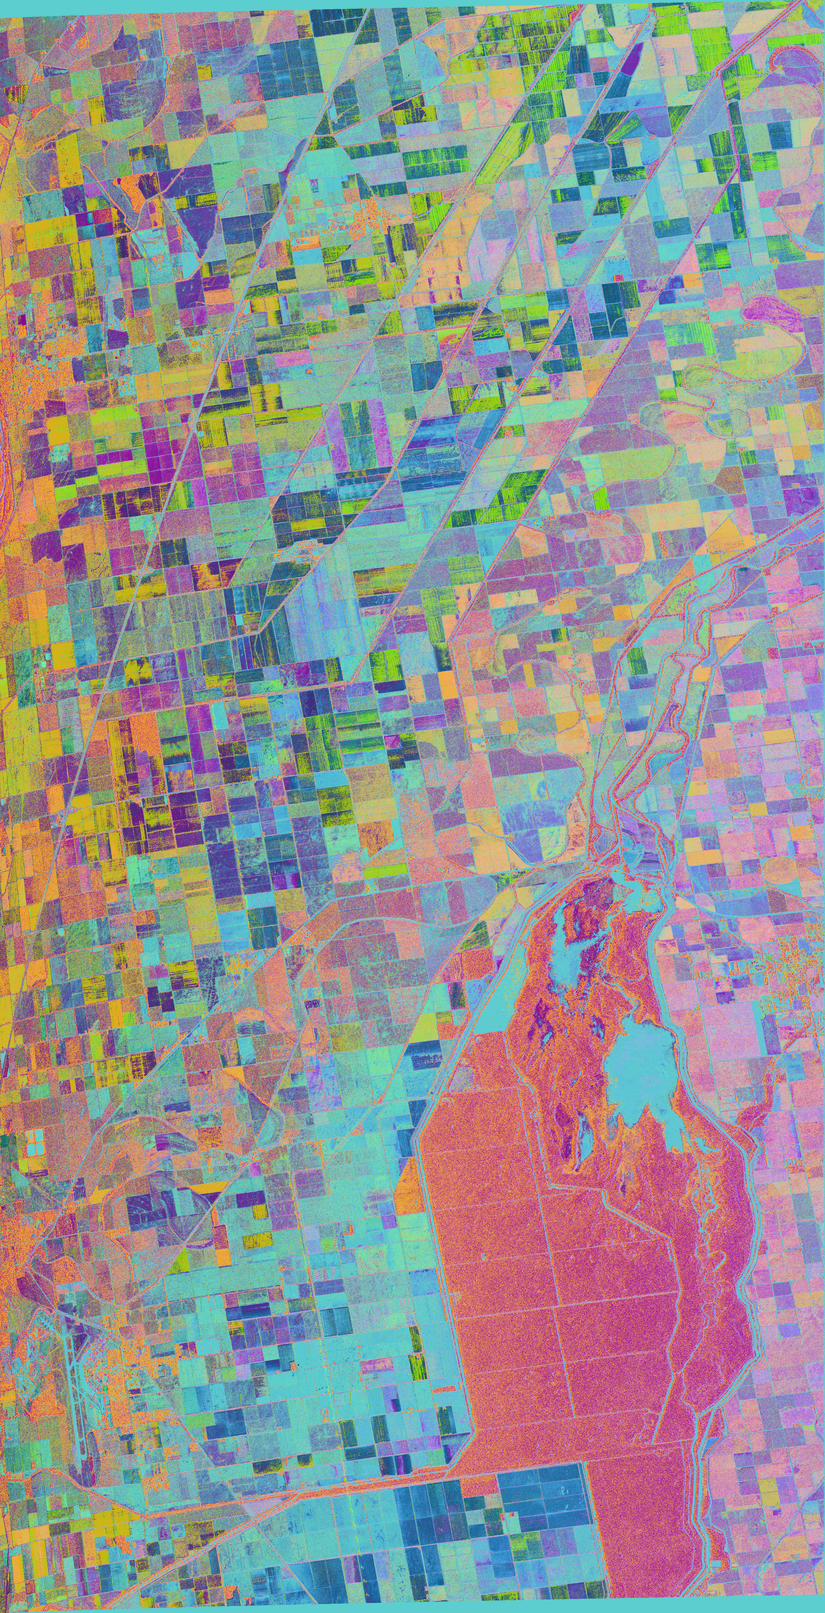
\includegraphics[width=.24\linewidth,viewport=575 600 825 850,clip]{../image/pauli_decorr}}
\subcaptionbox{Equalized zoom\label{Im:ZoomEqualized}}{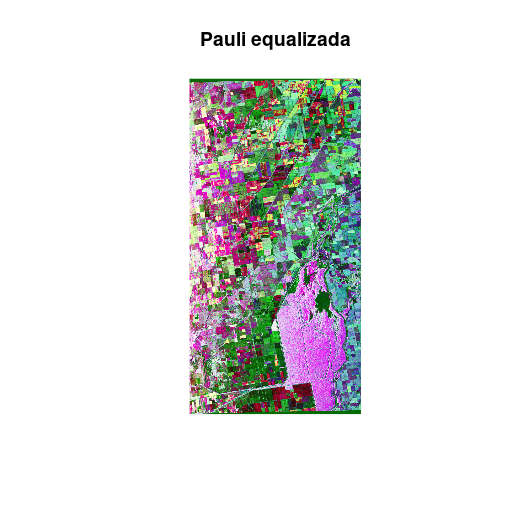
\includegraphics[width=.24\linewidth,viewport=575 600 825 850,clip]{../image/pauli_equalizada}}
\subcaptionbox{Enhanced zoom\label{Im:ZoomImproved}}{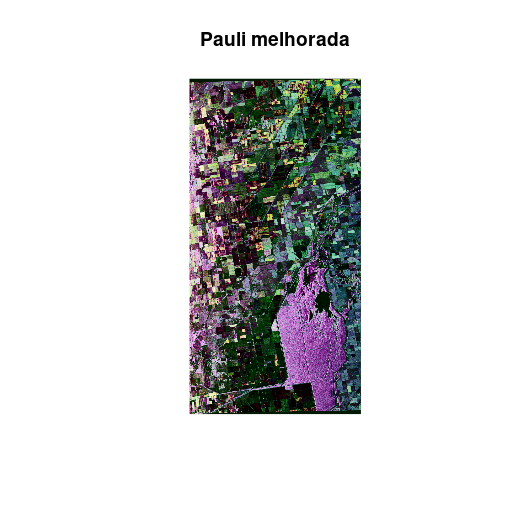
\includegraphics[width=.24\linewidth,viewport=575 600 825 850,clip]{../image/pauli_melhorada}}
\caption{Original Pauli, enhanced by decorrelation, equalized, and enhanced images, along with their zooms}\label{Fig:Images}
\end{figure*}

\section{DISCUSSION}
\label{sec:typestyle}
We have presented an image enhancement technique which preserves the chroma and hue.
The transformation is based on pixel-wise operations, and requires a reference image that is fixed for every application and input image size.
The results suggest that preserving the chroma and hue is a relevant feature, in particular for the visual interpretation of polarimetric decompositions.

We suggest adding this transformation, and its associated measure of performance, to visualization pipelines.

\bibliographystyle{IEEEtranSN}
\bibliography{../references}

\end{document}
